\chapter{Training Multi-Agent Reinforcement Learning Policies for Crazyflie Quadrotors}

This chapter presents our methodology for training decentralized \gls{marl} policies that enable a team of Crazyflie quadrotors to cooperatively transport a cable-suspended payload. We begin by formulating the cooperative transport task as a \gls{dec-pomdp}, defining the state, action, observation, and reward structures. We then describe our high-performance simulation and training pipeline, \todo{write method intro}
\section{Problem Formulation}

We model a team of $N$ Crazyflie quadrotors collaboratively carrying a cable-suspended payload as the Dec-POMDP $(\mathcal{N}, \mathcal{S}, \{\mathcal{A}^i\}_{i=1}^N, P, r, \{\Omega^i\}_{i=1}^N, O, \gamma)$, where $\mathcal{N} = \{1,2,\dots,N\}$ is the set of agents. At each discrete timestep $t$, the global state 
\[
s_t = \bigl(\{\mathbf{p}^i_t,\mathbf{v}^i_t,\mathbf{R}^i_t,\boldsymbol{\omega}^i_t\}_{i=1}^N,\; \mathbf{p}^P_t,\mathbf{v}^P_t\bigr)
\]
encapsulates each quadrotor's position $\mathbf{p}^i_t \in \mathbb{R}^3$, velocity $\mathbf{v}^i_t \in \mathbb{R}^3$, attitude $\mathbf{R}^i_t \in SO(3)$, angular velocity $\boldsymbol{\omega}^i_t \in \mathbb{R}^3$, and the payload's position $\mathbf{p}^P_t \in \mathbb{R}^3$ and velocity $\mathbf{v}^P_t \in \mathbb{R}^3$. The transition model $P(s_{t+1}\mid s_t, a_t)$ corresponds to a single simulation step in MuJoCo MJX, which approximates the continuous quadrotor–payload dynamics (including cable tensions and disturbances) over the fixed interval $\Delta t$.

Each agent $i$ selects an action 
\[
a^i_t = (f^i_{1,t},f^i_{2,t},f^i_{3,t},f^i_{4,t}) \in \mathbb{R}^4
\]
where $f^i_{j,t}$ is the thrust of rotor~$j$. The joint action is $a_t = (a^1_t,\dots,a^N_t)$. 

We define the payload position tracking error as
$
\mathbf{e}^P_t \;=\; \mathbf{p}^P_t \;-\; \mathbf{p}^P_{\mathrm{des},t},
$
so that $\|\mathbf{e}^P_t\|^2$ represents the squared tracking error at time $t$. A shared reward 
\[
r(s_t,a_t) = -\,\|\mathbf{e}^P_t\|^2 \;-\; \text{(stability penalties)}
\]
penalizes payload tracking error $\|\mathbf{e}^P_t\|^2$ and includes additional terms to discourage large payload swing or cable-tension imbalance.

Agent $i$ observes 
\[
o^i_t = \bigl(\hat{\mathbf{p}}^i_t,\hat{\mathbf{v}}^i_t,\hat{\mathbf{R}}^i_t,\hat{\boldsymbol{\omega}}^i_t,\mathbf{e}^P_t,\mathbf{v}^P_t\bigr),
\]
where $\hat{\mathbf{p}}^i_t,\hat{\mathbf{v}}^i_t,\hat{\mathbf{R}}^i_t,\hat{\boldsymbol{\omega}}^i_t$ are EKF estimates of its own state and $\mathbf{e}^P_t,\mathbf{v}^P_t$ are the payload state from motion capture. The observation function $O(o^i_t \mid s_t)$ models sensor noise and maps the global state $s_t$ to each $o^i_t$. Finally, $\gamma \in [0,1)$ is the discount factor.

Each agent $i$ maintains a policy $\pi^i_{\theta_i}(a^i \mid \tau^i)$ conditioned on its action-observation history $\tau^i_t = (o^i_0,a^i_0,\dots,o^i_t)$. During decentralized execution, the joint policy factorizes as
\[
\pi_\theta(a_t \mid \tau_t) \;=\; \prod_{i=1}^N \pi^i_{\theta_i}(a^i_t \mid \tau^i_t),
\]
where $\theta=(\theta_1,\dots,\theta_N)$. We seek $\theta$ that maximizes the expected discounted return
\[
J(\theta) = \mathbb{E}\Bigl[\sum_{t=0}^\infty \gamma^t\,r(s_t,a_t)\Bigr],
\]
subject to $s_{t+1}\sim P(\cdot\mid s_t,a_t)$, $a^i_t\sim \pi^i_{\theta_i}(\cdot\mid \tau^i_t)$, and $o^i_t\sim O(\cdot\mid s_t)$. By maximizing $J(\theta)$, agents learn to jointly minimize payload tracking error $\|\mathbf{e}^P_t\|^2$ while maintaining stability throughout the cooperative transport task.
\section{CrazyMARL}
We present \textbf{CrazyMARL}, an end-to-end JAX-based pipeline for training multi-agent reinforcement learning (MARL) policies on teams of Crazyflie quadrotors. Our framework seamlessly handles both single-vehicle and cooperative multi-agent tasks, including scenarios with cable-suspended payloads. At its core, the simulation leverages the high-performance MJX backend of the MuJoCo physics engine \cite{todorov_mujoco_2012}, interfaced through the Brax library for highly parallelized training. Our environments and algorithms are based on JaxMARL introduced by \autocite{flair2023jaxmarl}. We expose the simulator as a \texttt{JAXMARL.Mabrax} environment, providing a drop-in API for JAX-based RL algorithms.
\autocite{gymnax2022github} based on gymnax.
\subsection{Simulation Environment}
The simulation environment is built upon MuJoCo's XML specification and the GPU-accelerated MJX solver. We adopt a modular, extensible design in which each scenario is defined by auto-generated XML descriptors. These files specify vehicle geometries, inertial properties, cable parameters, payload characteristics, and any static or dynamic obstacles. A lightweight Python utility reads a user-defined configuration (YAML or JSON) and generates the corresponding XML, allowing researchers to rapidly prototype new dynamics or collaborative tasks. \todo{more details on configuration and generation of the XML files.}




\subsubsection{Quadrotor}
% - Modeling of quadrotor with thrust based on work of https://github.com/google-deepmind/mujoco_menagerie/blob/main/bitcraze_crazyflie_2/cf2.xml
- Describe thrust on quadrotor
- Motor Model

\subsubsection{Cable Suspended Payload}
- Description of cable suspended payload modeling with tendons or cables
% \subsubsection{Obstacles}
\subsubsection{Simulation Parameters}
- Configuration of simulation with initial position wind etc

\subsection{Observation Space}

At each control step \(t\), the simulation environment produces a high-dimensional state vector. We map this to a global observation vector 
\[
\mathbf{o}_t \;=\; \bigl[\;\underbrace{\mathbf{e}^P_t}_{3},\;\underbrace{\mathbf{v}^P_t}_{3},\;\underbrace{\{\;\mathbf{r}^i_t,\;\mathrm{vec}(\mathbf{R}^i_t),\;\mathbf{v}^i_t,\;\boldsymbol{\omega}^i_t,\;\mathbf{a}^i_t,\;\boldsymbol{\alpha}^i_t\}_{i=1}^N}_{24N},\;\underbrace{\mathbf{a}_{t-1}}_{4}\bigr] \;\in\;\mathbb{R}^{6 + 24N + 4}
\]
Here \(\mathbf{e}^P_t = (\mathbf{p}^P_{\mathrm{des},t}-\mathbf{p}^P_t)/\max(\|\mathbf{p}^P_{\mathrm{des},t}-\mathbf{p}^P_t\|,1)\) is the normalized payload tracking error, and \(\mathbf{v}^P_t\) its velocity.  For each quadrotor \(i\), \(\mathbf{r}^i_t=\mathbf{p}^i_t-\mathbf{p}^P_t\) denotes its position relative to the payload, \(\mathrm{vec}(R^i_t)\in\mathbb{R}^9\) the row-major flattening of its rotation matrix, \(\mathbf{v}^i_t\) and \(\boldsymbol{\omega}^i_t\) its body-frame linear and angular velocities, \(\mathbf{a}^i_t\) and \(\boldsymbol{\alpha}^i_t\) its body-frame linear and angular accelerations and \(\mathbf{a}_{t-1}\) the concatenation of all agents previous thrust commands.  By construction, this global observation vector contains all information required to compute rewards and termination conditions.

During decentralized execution, each agent \(i\) receives only the subset of entries corresponding to the payload terms, its own dynamic state block, and its most recent command.  Concretely, agent \(i\) observes
\[
\mathbf{o}^i_t 
\;=\;
\bigl[\,
\mathbf{e}^P_t,\;\mathbf{v}^P_t,\;\mathbf{r}^i_t,\;\mathrm{vec}(\mathbf{R}^i_t),\;\mathbf{v}^i_t,\;\boldsymbol{\omega}^i_t,\;\mathbf{a}^i_t,\;\boldsymbol{\alpha}^i_t,\;\mathbf{a}^i_{t-1}
\,\bigr]\;\in\;\mathbb{R}^{6 + 24 + 4}\,,
\]
so that each policy conditions on the payload's error and velocity, the agent's full pose and inertial measurements, and its previous action.  This restriction enforces the Dec-POMDP structure, by hiding other agents' internal states, coordination must emerge through the shared reward alone.

\subsection{Action Space}

Each agent \(i\) outputs a four-dimensional vector \(\tilde{\mathbf{a}}^i_t\in[-1,1]^4\), representing normalized thrust commands for its rotors.  These are mapped to physical rotor forces via
\[
f^i_{j,t}
\;=\;
\frac{\tilde{a}^i_{j,t} + 1}{2}\;f_{\max}^i,
\qquad
j=1,\dots,4,
\]
where \(f_{\max}^i\) is the agent-specific maximum thrust, randomly perturbed at the start of each episode to improve robustness.  Optionally, zero-mean Gaussian noise proportional to \(f_{\max}^i\) may be added to each \(f^i_{j,t}\) to model actuator uncertainty.  The resulting thrust vector \(\mathbf{f}^i_t\) is then applied in the physics simulator, yielding continuous next-state dynamics.  

By constraining \(\tilde{\mathbf{a}}^i_t\in[-1,1]^4\) and sampling \(f_{\max}^i\) within a known bound, the policy learns to produce smooth, safe thrust profiles that transfer effectively from simulation to the real Crazyflie platform.  
\subsection{Domain Randomization}
\subsubsection{Environment Reset}
\todo{reset fig}
\label{sec:reset}
\begin{figure}
    \centering
    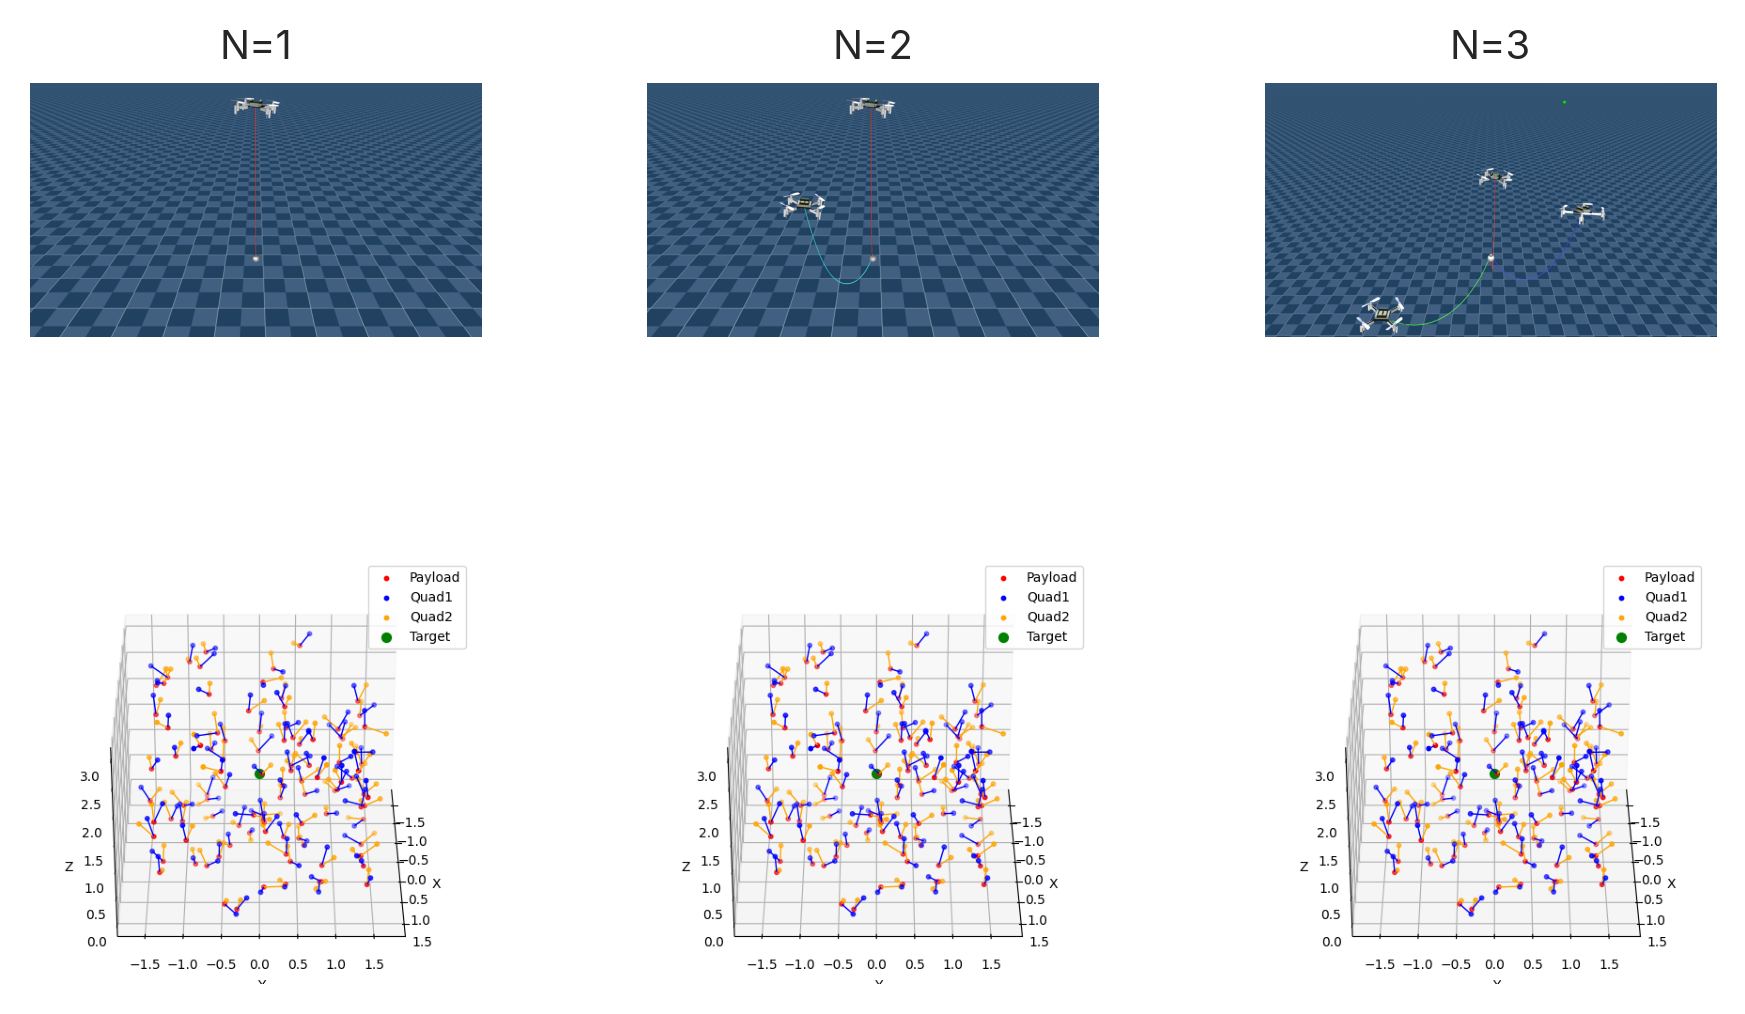
\includegraphics[width=\textwidth]{experiments/initial_conditions.png}
    \caption[Harsh conditions generation]{Randomly sampled initial configurations for the payload and quadrotors. The payload is positioned at the center, while quadrotors are uniformly distributed in a spherical shell around it.}
    \label{fig:reset_config}
\end{figure}
At each reset, the payload center~$p$ is sampled uniformly in
\[
p_{xy}\sim\mathcal{U}([-L,L]^2),\quad p_z\sim\mathcal{U}([-Z,Z]),
\]
Then we use the payload position $p$ as the center point and randomly sample $N$ quadrotors in a spherical shell around the payload. The radius $r_i$ of each quadrotor is sampled from a normal distribution with mean $\mu_r$ and standard deviation $\sigma_r$, and then clipped to cable length. The angles $\theta_i$ and $\phi_i$ are sampled from normal distributions with means $\mu_\theta$ and $\phi_{\mathrm{offset}}$ respectively, and standard deviations $\sigma_\theta$ and $\sigma_\phi$. The angles are then adjusted to ensure they are within the range $[0, 2\pi]$. The equations for sampling the quadrotor positions are as follows:
\[
r_i = \mathrm{clip}\bigl(\mu_r+\sigma_r\varepsilon_i^{(r)},\,r_{\min},\,r_{\max}\bigr),\quad
\theta_i = \mu_\theta+\sigma_\theta\varepsilon_i^{(\theta)},\quad
\phi_i = \tfrac{2\pi(i-1)}{N} + \phi_{\mathrm{offset}} + \sigma_\phi\varepsilon_i^{(\phi)},
\]
where $\varepsilon_i^{(\cdot)}\!\sim\mathcal{N}(0,1)$, $\phi_{\mathrm{offset}}\!\sim\mathcal{U}(-\pi,\pi)$, and
\[
\mu_r=c,\;\sigma_r=\tfrac{c}{3},\;r_{\min}=0.05,\;r_{\max}=c,\;
\mu_\theta=\tfrac{\pi}{7},\;\sigma_\theta=\tfrac{\pi}{8},\;\sigma_\phi=\tfrac{\pi}{N+1}.
\]

These are converted to Cartesian positions
\[
q_i = p + r_i
\begin{bmatrix}
\sin\theta_i\cos\phi_i\\
\sin\theta_i\sin\phi_i\\
\cos\theta_i
\end{bmatrix},
\]
\todo{fix equations}
with the $z$–coordinate clipped. 
This results in a even distribution of valid initial configurations, also including starting from the ground as shown in \autoref{fig:reset_config}. 



\subsubsection{Hardeware Rollout}




\subsection{Reward Design}
\todo{update reward}
\todo{split quad reward -> payload reward}
The goal of our reward is to encourage flight behaviors that bring the payload to its target at a speed of roughly $ v_{\max} = 0.7m/s$, while simultaneously minimizing payload swing and vehicle tilt, maintaining a taut suspension cable, enforcing safe spacing between quadrotors, and promoting gentle, low-frequency thrust commands for robust sim-to-real transfer. Harsh penalties can induce “learning to terminate” behaviors or unstable gradients. In order to prevent this, we shape all error components with the bounded exponential function

\[
\rho(x; s) \;=\;\exp\bigl(-s\,|x|\bigr)\;-\;0.1\,s\,|x|\,,\quad s>0,
\]
and inject a small constant \(\varepsilon>0\) wherever needed to prevent division by zero.

\subsubsection{Payload Tracking and Velocity Alignment}
Define the payload position error \(\mathbf{e}^P_t = \mathbf{p}^P_t - \mathbf{p}^P_{\mathrm{des},t}\) with norm \(d_t = \|\mathbf{e}^P_t\|\).  The payload velocity is \(\mathbf{v}^P_t\).  We scale velocity conditioned on the distance and set
\[
v_{\mathrm{des}}(d_t)
= v_{\max}\bigl(1 - e^{-8\,d_t}\bigr),\quad
\]
and measure the velocity error
\[
\Delta v_t
= \Bigl\|\mathbf{v}^P_t - v_{\mathrm{des}}(d_t)\,\frac{\mathbf{e}^P_t}{d_t + \varepsilon}\Bigr\|.
\]
The raw tracking reward
\[
\tilde r_{\mathrm{track}}
= 2
\;+\;\rho\bigl(d_t; s_d\bigr)
\;+\;\rho\bigl(\Delta v_t; s_v\bigr)
\]
is clipped at zero to yield
\[
r_{\mathrm{track}}=\max\{0,\tilde r_{\mathrm{track}}\},
\]
ensuring only positive incentive remains.

\subsubsection{Inter-Agent Safe-Distance}
For \(N>1\) quadrotors with planar positions \(\mathbf{p}^i_{t,xy}\), let
\[
d_{ij} = \lVert\mathbf{p}^i_{t,xy}-\mathbf{p}^j_{t,xy}\rVert,\quad i\neq j.
\]
We reward the normalized sum
\[
r_{\mathrm{safe}}
= \frac{1}{N(N-1)}\sum_{i\neq j}\mathrm{clip}\!\Bigl(\tfrac{d_{ij}-d_{\min}}{w_d},0,1\Bigr),
\]
which scales naturally with \(N\). The default \(d_{\min}=0.15\) and \(w_d=0.02\) ensure a minimum safe distance of 15 cm between quadrotors, with a linear penalty for closer approaches.

\subsubsection{Uprightness}
Tilt angles \(\theta^i_t\) between each quad's body-frame “up” axis and gravity are shaped by
\[
r_{\mathrm{up}}
= \frac{1}{N}\sum_{i=1}^N \rho\bigl(\theta^i_t; s_\theta\bigr),
\]
discouraging large roll or pitch that induce instability and payload swing.

\subsubsection{Taut-String Maintenance}
Let \(d^i_t=\lVert\mathbf{p}^i_t-\mathbf{p}^P_t\rVert\) and \(h^i_t=(\mathbf{p}^i_t)_z-(\mathbf{p}^P_t)_z\).  A taut cable of length \(L\) is encouraged by maximizing both terms via
\[
r_{\mathrm{taut}}
= \frac{1}{L}\Bigl(\frac{1}{N}\sum_{i=1}^N d^i_t + \frac{1}{N}\sum_{i=1}^N h^i_t\Bigr).
\]

\subsubsection{Rotor-Frame Velocity Regularization}
For each quad's body-frame angular velocity \(\boldsymbol{\omega}^i_t\) and linear velocity \(\mathbf{v}^i_t\), we define
\[
r_{\omega}
= \frac{1}{N}\sum_{i=1}^N \rho\bigl(\lVert\boldsymbol{\omega}^i_t\rVert; s_\omega\bigr),
\quad
r_{v}
= \frac{1}{N}\sum_{i=1}^N \Bigl[\rho\bigl(\lVert\mathbf{v}^i_t\rVert; s_v\bigr)
- c_v\,\mathrm{clip}\bigl(\lVert\mathbf{v}^i_t\rVert - v_{\max},0,\infty\bigr)\Bigr].
\]

\subsubsection{Collision and Boundary Penalties}
With indicators \(\mathbb{I}_{\mathrm{coll}}\), \(\mathbb{I}_{\mathrm{oob}}\) and a grace factor \(g(t)=\mathrm{clip}(2t,0,1)\), penalties are
\[
r_{\mathrm{coll}} = -\,g(t)\,\mathbb{I}_{\mathrm{coll}}, 
\quad
r_{\mathrm{oob}} = -\,g(t)\,\mathbb{I}_{\mathrm{oob}}.
\]

\subsubsection{Smoothness and Energy Cost}
\begin{figure}[ht]
    \centering
    
    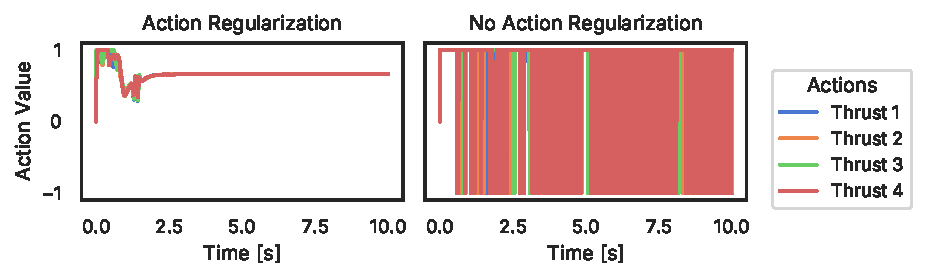
\includegraphics[width=\textwidth]{experiments/actions_comparison.pdf}
    \caption[Policy comparison with/without action regularization]{Comparison of policy trained with and without the action regularization reward. The left plot shows the actions over time of the policy with regularization, while the right plot shows the actions of the policy without regularization. The regularized policy produces smoother and more stable actions, while the unregularized policy exhibits large fluctuations in thrust commands jumping between the action limits.}
    \label{fig:}
\end{figure}
Let \(\mathbf{a}_t,\mathbf{a}_{t-1}\) be consecutive normalized thrust vectors and \(\tilde f_{i,j}\) each rotor's thrust fraction.  We set
\[
r_{\mathrm{smooth}}
= -\sum_{i,j} \bigl|a_{t,i,j}-a_{t-1,i,j}\bigr|,
\quad
r_{\mathrm{energy}}
= -\frac{1}{4N}\sum_{i=1}^N\sum_{j=1}^4\bigl[\exp\bigl(-30|\tilde f_{i,j}|\bigr)+\exp\bigl(90(\tilde f_{i,j}-1)\bigr)\bigr].
\]
The energy cost discourages thrust to be on the limits at 0 or 1, while the smoothness term penalizes large changes in thrust between consecutive timesteps, promoting stable flight.
\subsubsection{Aggregate Reward}
The stability incentive is the average of its five components:
\[
r_{\mathrm{stab}}
= \frac{1}{5}\bigl(r_{\mathrm{safe}} + r_{\mathrm{up}} + r_{\mathrm{taut}} + r_{\omega} + r_{v}\bigr),
\]
and the total penalty is
\[
r_{\mathrm{pen}}
= r_{\mathrm{coll}} + r_{\mathrm{oob}} + r_{\mathrm{smooth}} + r_{\mathrm{energy}}.
\]
Finally, we multiply tracking and stability to enforce simultaneous performance,
\[
r_t
= r_{\mathrm{track}}\;r_{\mathrm{stab}}
\;+\;r_{\mathrm{pen}}.
\]
This product structure ensures the policy learns to track the payload while constantly maintaining stable formations, and the additive penalties discourage unsafe or aggressive behaviors without overwhelming the shaping incentives.

\subsection{Reward Design Considerations}
\todo{write reward design considerations}
\subsection{Integration with JAXMARL}

CrazyMARL integrates seamlessly with the JaxMARL ecosystem \cite{flair2023jaxmarl}.  We wrap each Brax environment in a \texttt{JAXMARL.Mabrax} adapter, exposing standard methods for rollout collection, batching, and replay buffer storage.  The same RL algorithms (e.g., PPO, QMIX) can be applied unchanged to single-agent or decentralized multi-agent tasks, enabling rapid experimentation across a broad class of cooperative aerial transport problems.


\section{Training}
\begin{figure}[ht]
    \centering
    
    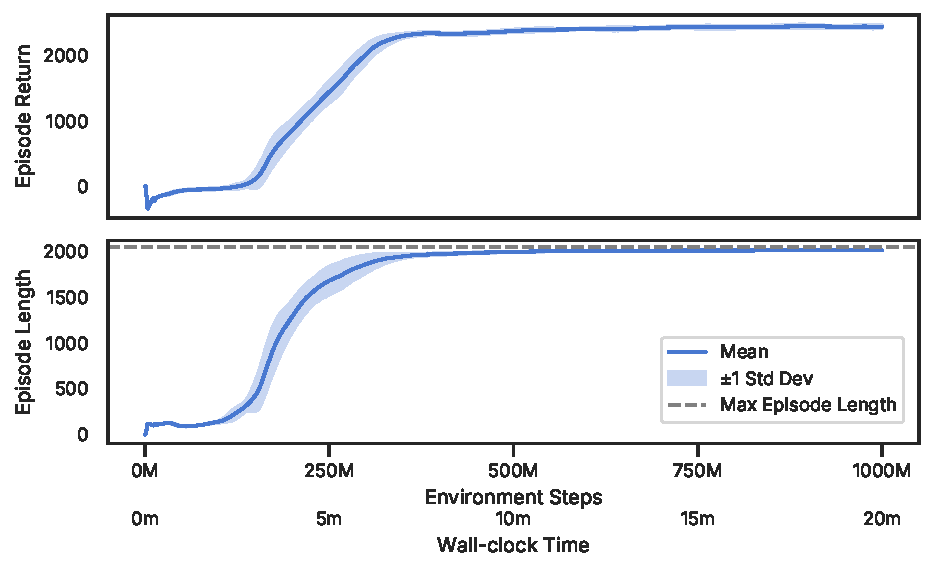
\includegraphics[width=\textwidth]{experiments/train_metrics.pdf}
    \caption[Training metrics]{Average training metrics for one quadrotor with payload scenario. The top plot shows the average episode returns and the bottom plot shows the average episode lengths over environment steps and wall-clock time. The shaded area represents the standard deviation across 10 seeds. The maximum possible episode lenght here is 2048 environment steps, which corresponds to 8.2 seconds of flight time. In the end nearly all episodes are completing the episode indicating stable flight.}
    \label{fig:train_metrics}
\end{figure}
\todo{add training metrics comparison}
Our training pipeline follows the approach of \autocite{flair2023jaxmarl}, leveraging the JaxMARL framework to implement decentralized policy optimization. We use the \gls{ippo} algorithm, which extends \gls{ppo} to multi-agent settings by optimizing a joint policy across all agents while maintaining decentralized execution.

The decentralized policies are learned end-to-end via \gls{ppo} within our highly parallelized JAX/MJX simulation environment. At each iteration, a fixed number of synchronous actors collect trajectories in $M$ parallel environments over $N$ time steps, yielding $NM$ experiences per update. Collected rewards are bootstrapped with the learned critic to compute targets, and advantages are estimated using \gls{gae} with discount factor $\gamma$ and smoothing parameter $\lambda$. The overall loss combines the clipped policy objective
\[
L_{\mathrm{PPO}}(\theta) = \mathbb{E}\!\bigl[\min\bigl(r_t(\theta)\,\hat{A}_t,\;\mathrm{clip}(r_t(\theta),1-\epsilon,1+\epsilon)\,\hat{A}_t\bigr)\bigr],
\]
a mean-squared value-function error, and an entropy regularizer to encourage sufficient exploration. Gradient norms are clipped to enhance numerical stability.

\subsection{Policy Architecture}
Both actor and critic networks are instantiated as fully connected, feed-forward multilayer perceptrons. The actor network comprises an input layer matching the local observation dimension, three hidden layers of 64 units with tanh activations, and a linear output layer producing the action-mean vector. A learned log-standard deviation vector of the same dimensionality parameterizes a diagonal Gaussian policy. The critic network features three hidden layers of 128 tanh units each, terminating in a scalar output. All dense layers employ orthogonal weight initialization and zero biases. During training and rollouts, actions are sampled stochastically from the policy distribution, at evaluation time, the deterministic mean action is used.

\subsection{Optimization and Hyperparameters}
We run a baysian optimization sweep over the hyperparameters to find the best configuration for our task. Initially running a coarse search over a wide range of values, we then refine the search around promising regions. The final hyperparameters are selected based on the best performance.

% \subsubsection{Comparing Centralized PPO, IPPO, and MAPPO}
% We compare three variants of the \gls{ppo} algorithm: centralized \gls{ppo}, decentralized \gls{ippo}, and multi-agent \gls{mappo}. The centralized variant uses a shared critic for all agents, while \gls{ippo} and \gls{mappo} maintain decentralized policies with independent critics. 
% \begin{itemize}
%     \item 3 Plots with training (episode-length over steps) with 3 different seeds each
% \end{itemize}

